\documentclass[../../DD.tex]{subfiles}
\begin{document}
\newpage
\subsection{Kind of Topic}
	\subsubsection{Our Team}
		\textit{Our Team} page contains all the people who works for \textit{VenTour}.\\
        People are divided in four different teams, that are described in the four cards at the top of the page.\\
        Every person is contained in a card with his/her photo and name. When the user's cursor hovers over a card, role and area of responsibility also appear in the same place. The user can click on a card to access to the person's dedicated page.\\
        People can be filtered by department in the same page.\\
        The user can access to \textit{Investment} page by clicking on "Check our Investments" button.\\
        Everything described can be seen in figure \ref{fig: Our_team_screen}
        \newline

\begin{figure}[!htb]
      \centering
      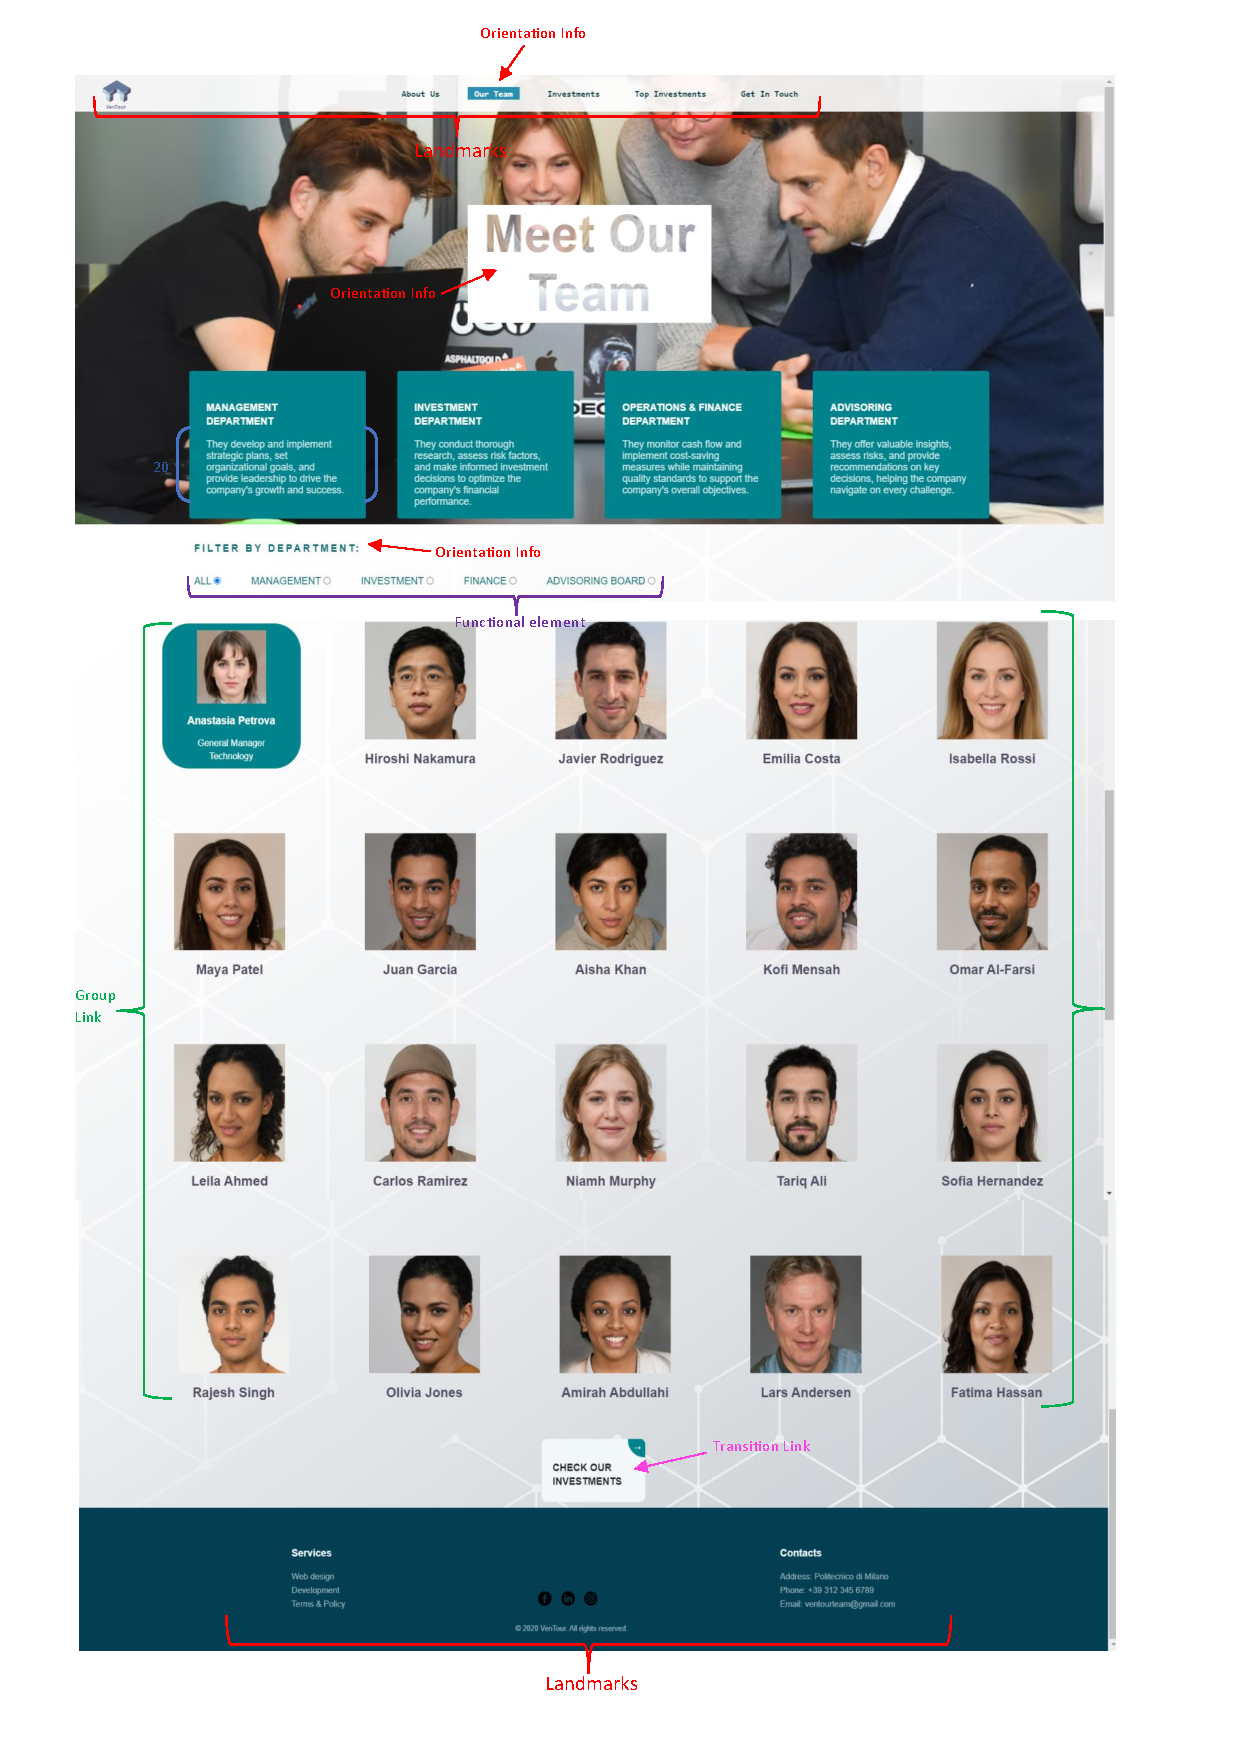
\includegraphics[width=0.9\textwidth]{Images/screenshots/Our Team_screen.pdf}
      \caption{Our Team page}
      \label{fig: Our_team_screen}
  \end{figure}

\newpage
	\subsubsection{Investments}
		\textit{Investments} page contains the list of all investment areas of our venture company, in the first section and all investments(companies),in the second section. They can be accessible from their specific group links.\\
  The page offers the possibility to filter the companies, according to the area chosen by clicking first the functional elements and then the buttons, which function as structural links. An additional option is to search each company by its name from the input box found on top of the Portfolio Snapshot.\\
  The third section of the page is dedicated to the exit strategies of our company. Structural links make possible the navigation between these strategies. 
  \begin{figure}[!htb]
      \centering
      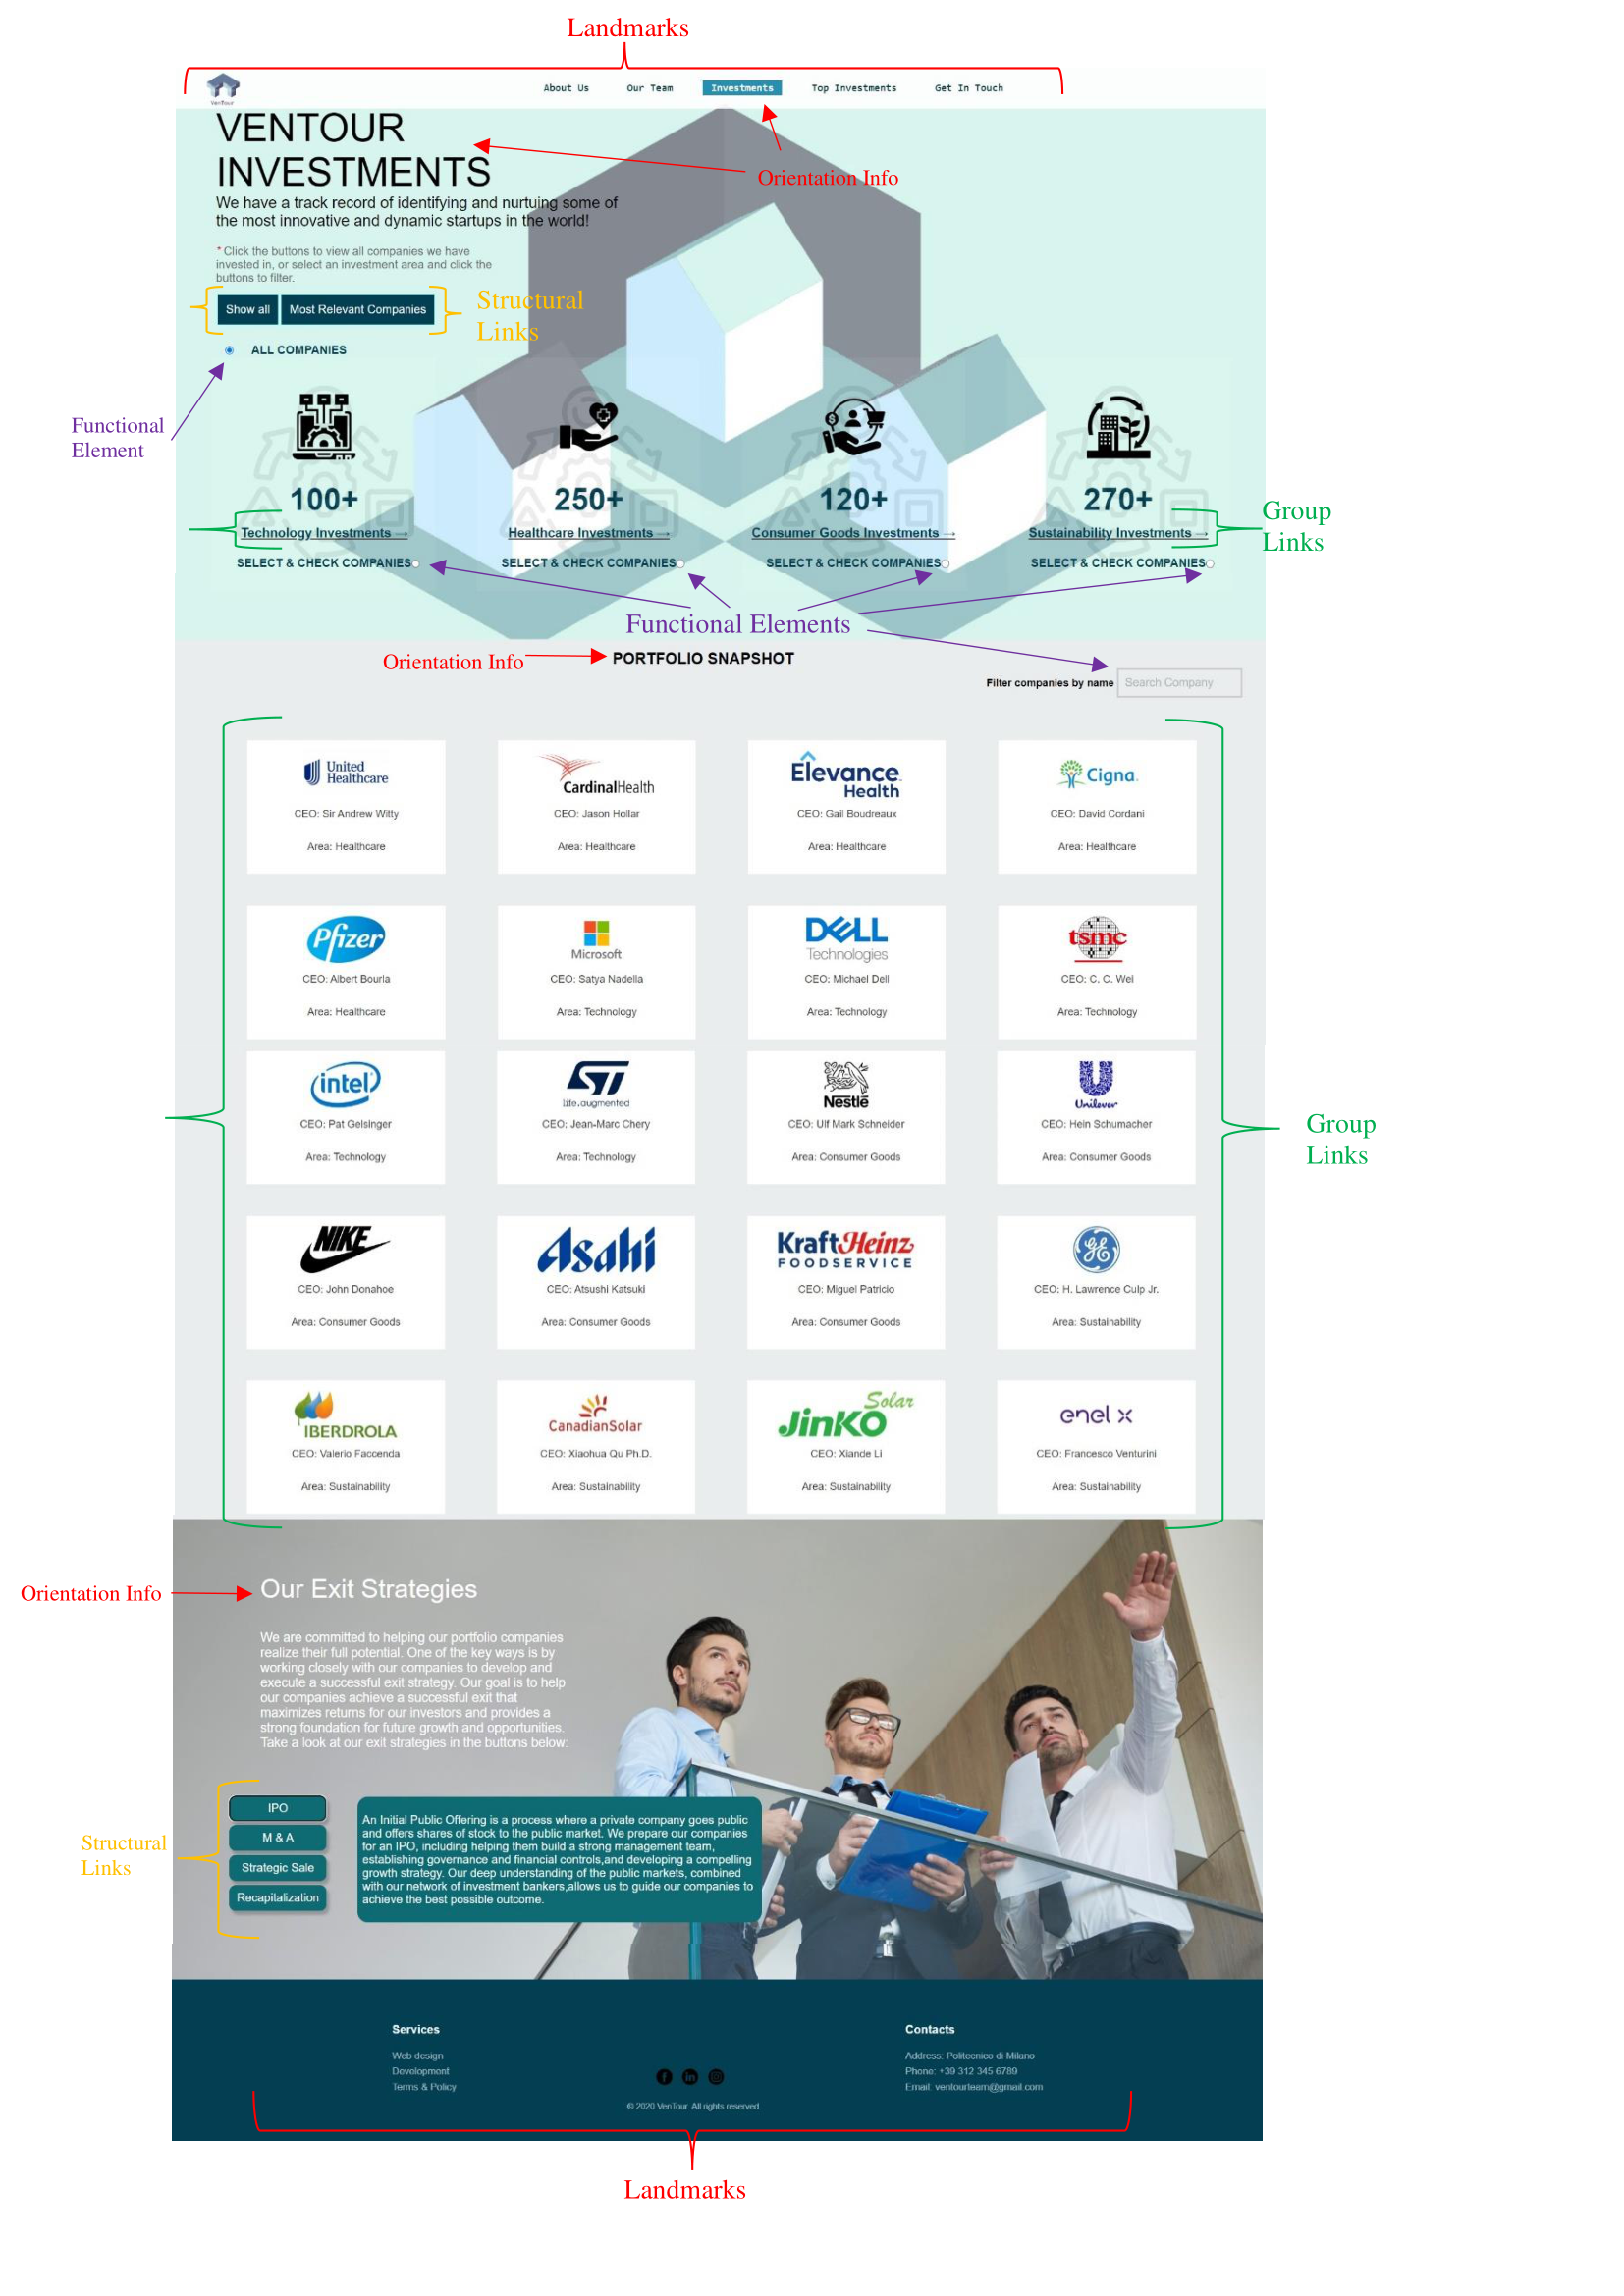
\includegraphics[width=0.95\textwidth]{Images/screenshots/investments scr.png}
      \caption{Investments Page screenshot}
      \label{fig:investments-screenshot}
  \end{figure}
	%\newpage
	\subsubsection{Area of investment}
		Single \textit{Area} page represents the investment area at which our company is developing investments. There are in total 4 areas: Technology, Healthcare, Consumer Goods and Sustainability, all represented with a page design as shown below.\\
        The page is divided in two sections. The first section contains the title, which is the area name, an image and a description of the \textit{Investment Area}. In the second section below , transition links to the \textit{Companies}, included in the specific area, are presented with a slider of cards.
		\newline
		\image{\textheight}{screenshots/area scr.png}{Area of Investment page screenshot}{area-screenshot}
\newpage
	\subsubsection{Top Investments}
		\textit{Top Investments} page includes the most relevant investments, which are part of the total investments. Until now our company has 4 top investments, one for each investment area.\\ These investments (companies) are put in a carousel of images that are clickable and from which the page of the specific company can be reached.\\
        Below the carousel, a button links to all investments.
		\newline
		\image{\textheight}{screenshots/topinv scr.png}{Area of Investment page screenshot}{AreaOfInv-screenshot}
	

\end{document}
